\documentclass[12pt]{article}

\usepackage{sbc-template}
\usepackage{graphicx,url}
\usepackage[utf8]{inputenc}
\usepackage[brazil]{babel}
%\usepackage[latin1]{inputenc}  

\usepackage{indentfirst}
\setlength{\parindent}{1.25cm}
     
\sloppy

\title{A Evolução do Armazenamento Secundário: Uma Revisão de Literatura das Tecnologias HDD vs. SSD (NVMe, TRIM e TBW)}

\author{Etelvina Ellen G. Torres\inst{1}, Heloiza Graziele P. Amaro\inst{1}, Walter Felipe dos Santos\inst{1}}

\address{Universidade Federal do Vale do São Francisco - UNIVASF\\
    Bacharelado em Ciência da Computação\\
Salgueiro -- PE -- Brasil
\email{\{etelvina.torres, heloiza.g\} @discente.univasf.edu.br, walter.felipe@univasf.edu.br}
}

\usepackage{tabularx}
\usepackage{array}
\usepackage{float}
\raggedbottom

\begin{document} 

\maketitle
     
\begin{resumo} 
 O armazenamento secundário influencia o desempenho, a capacidade e a eficiência dos computadores. Este artigo apresenta uma revisão bibliográfica qualitativa sobre a evolução das tecnologias de armazenamento, comparando HDDs e SSDs, com ênfase nas interfaces SATA/AHCI e PCIe/NVMe e nos mecanismos de gerenciamento da memória Flash NAND. A análise considera latência, taxa de transferência, filas de comandos, custo por capacidade e durabilidade. Os resultados indicam que os SSDs NVMe apresentam vantagens de desempenho em relação aos HDDs e SSDs SATA, principalmente pela menor latência e pelo processamento paralelo de requisições. Entretanto, a memória Flash possui limitações nos ciclos de escrita e apagamento, exigindo mecanismos como TRIM, Garbage Collection e Wear Leveling, além da métrica TBW para avaliar sua durabilidade. Conclui-se que a escolha da tecnologia deve considerar as necessidades de cada aplicação, buscando equilibrar desempenho, capacidade e custo.

\end{resumo}
\par
{\setlength{\leftskip}{0.7cm}
\noindent\textbf{Palavras-chave:} \textit{Armazenamento secundário, HDD, SSD, NVMe, Memória \\
Flash NAND.}\par}

\begin{abstract}
Secondary storage influences the performance, capacity, and efficiency of computers. This article presents a qualitative literature review on the evolution of storage technologies, comparing HDDs and SSDs, with an emphasis on SATA/AHCI and PCIe/NVMe interfaces, as well as the management mechanisms for NAND Flash memory. The analysis considers latency, throughput, command queuing, cost-per-capacity, and durability. The results indicate that NVMe SSDs offer performance advantages over HDDs and SATA SSDs, primarily due to lower latency and the parallel processing of requests. However, Flash memory has limitations regarding write and erase cycles, necessitating mechanisms such as TRIM, Garbage Collection, and Wear Leveling, in addition to the TBW (Total Bytes Written) metric for assessing durability. It is concluded that the choice of technology should take into account the requirements of each specific application, seeking a balance between performance, capacity, and cost.

\end{abstract}

\par
{\setlength{\leftskip}{0.7cm}
\noindent\textbf{Keywords:} \textit{Secondary storage, HDD, SSD, NVMe, NAND Flash memory.}\par}

\section{Introdução}

O armazenamento secundário é um componente essencial da arquitetura dos computadores, pois permite conservar dados e programas mesmo quando o sistema é desligado. Sua evolução está diretamente relacionada à necessidade de ampliar a capacidade de armazenamento e melhorar a velocidade de acesso às informações. Nesse cenário, os discos rígidos magnéticos (HDDs) e as unidades de estado sólido (SSDs) representam tecnologias com características distintas, que influenciam o desempenho e a organização dos sistemas computacionais \cite{stallings2017}.

Tradicionalmente, os HDDs são utilizados para armazenar grandes volumes de dados por meio de processos eletromecânicos de leitura e gravação em pratos magnéticos. Embora apresentem vantagens relacionadas ao custo por unidade de capacidade, seu funcionamento depende do movimento de componentes físicos, o que pode aumentar a latência e limitar o desempenho em operações que exigem acessos frequentes aos dados. Em contrapartida, os SSDs utilizam memória Flash NAND para realizar o armazenamento eletrônico, eliminando as partes móveis e proporcionando menores tempos de acesso. Entretanto, essas unidades também apresentam limitações relacionadas ao desgaste das células de memória e aos procedimentos internos necessários para a gravação e a manutenção dos dados \cite{silva2025}, \cite{stallings2017}.

Além das diferenças entre os meios físicos, a evolução do armazenamento secundário envolve mudanças nas interfaces e nos protocolos de comunicação. Os dispositivos que utilizam SATA, associados ao protocolo AHCI, apresentam limitações em comparação às unidades NVMe conectadas ao barramento PCI Express \textit{(PCIe)}. Desenvolvido para aproveitar as características das memórias não voláteis, o NVMe oferece suporte a múltiplas filas de comandos, favorecendo o processamento paralelo de requisições e ampliando as possibilidades de desempenho dos SSDs. Paralelamente, mecanismos como TRIM, Garbage Collection e Wear Leveling contribuem para o gerenciamento da memória Flash, enquanto a métrica TBW \textit {(Terabytes Written)} auxilia na caracterização da resistência do dispositivo às operações de escrita.

Diante desse contexto, este artigo tem como objetivo analisar a evolução tecnológica e arquitetural do armazenamento secundário, comparando HDDs, SSDs SATA e SSDs NVMe quanto ao funcionamento, à latência, à taxa de transferência, ao gerenciamento lógico e à durabilidade. Busca-se também discutir os principais gargalos dessas tecnologias e os compromissos entre desempenho, capacidade e custo, considerando suas implicações para diferentes aplicações computacionais.

Para alcançar esse objetivo, foi realizada uma pesquisa bibliográfica de abordagem qualitativa, organizada no formato de artigo de revisão de literatura \textit{(survey)}. O estudo fundamenta-se em referências da área de Arquitetura de Computadores e em trabalhos técnicos relacionados às tecnologias analisadas. Além desta introdução, o artigo apresenta a metodologia de pesquisa, a sistematização teórica das tecnologias de armazenamento, a análise crítica de seus gargalos arquiteturais e, por fim, as considerações finais.

\section{Metodologia de Pesquisa}
O presente estudo caracteriza-se como uma pesquisa bibliográfica de abordagem qualitativa no formato de artigo \textit{survey}, visando analisar a evolução tecnológica e arquitetural dos dispositivos de armazenamento secundário. A fundamentação teórica baseia-se na literatura acadêmica de Arquitetura de Computadores \cite{stallings2017} para estruturar os conceitos de hierarquia de memória, barramentos (SATA e PCIe) e fluxo de Entrada e Saída (E/S), combinada a artigos científicos e estudos de caso recentes que detalham a física dos pratos magnéticos, a arquitetura Flash NAND, o paralelismo do protocolo NVMe e os mecanismos lógicos de gerenciamento (\textit{TRIM}, \textit{Garbage Collection} e \textit{Wear Leveling}) \cite{santos2014, ribeiro2017, george2023, xu2015}. A sistematização dos dados permitiu a elaboração de um diagrama de hierarquia de hardware e de uma tabela comparativa autoral para embasar a análise dos gargalos do subsistema.

\section{Taxonomia e Sistematização Teórica} 

\subsection{Introdução e Contextualização do Fluxo de Armazenamento} 
Para entender a evolução do armazenamento secundário na arquitetura de computadores, é preciso analisar a trajetória do fluxo de dados desde o processador (CPU) e a memória principal até a gravação persistente na mídia de armazenamento. Historicamente, esse papel foi desempenhado por dispositivos eletromecânicos (HDDs), enquanto a transição para sistemas de estado sólido baseados em memória Flash NAND (SSDs) eliminou as partes móveis, alterando a dinâmica de entrada e saída (E/S) do subsistema de memória \cite{santos2014, stallings2017}. 

Nesse contexto, enquanto a tecnologia magnética se conecta ao sistema por meio de controladores e barramentos herdados como o SATA/AHCI \cite{silva2025}, os SSDs de alta performance exploram vias diretas pelo barramento PCI Express (PCIe) operando sob o protocolo NVMe \cite{george2023}. Para ilustrar a hierarquia envolvida nesse fluxo de dados, a Figura \ref{fig:hierarquia-hardware} apresenta o caminho percorrido nas tecnologias mecânica e de estado sólido. 
%tem que colocar  referência a figura

\subsection{Diagrama Conceitual da Arquitetura e Hierarquia de Hardware} 


\begin{figure}[H]
\vspace{-6pt}
    \centering
    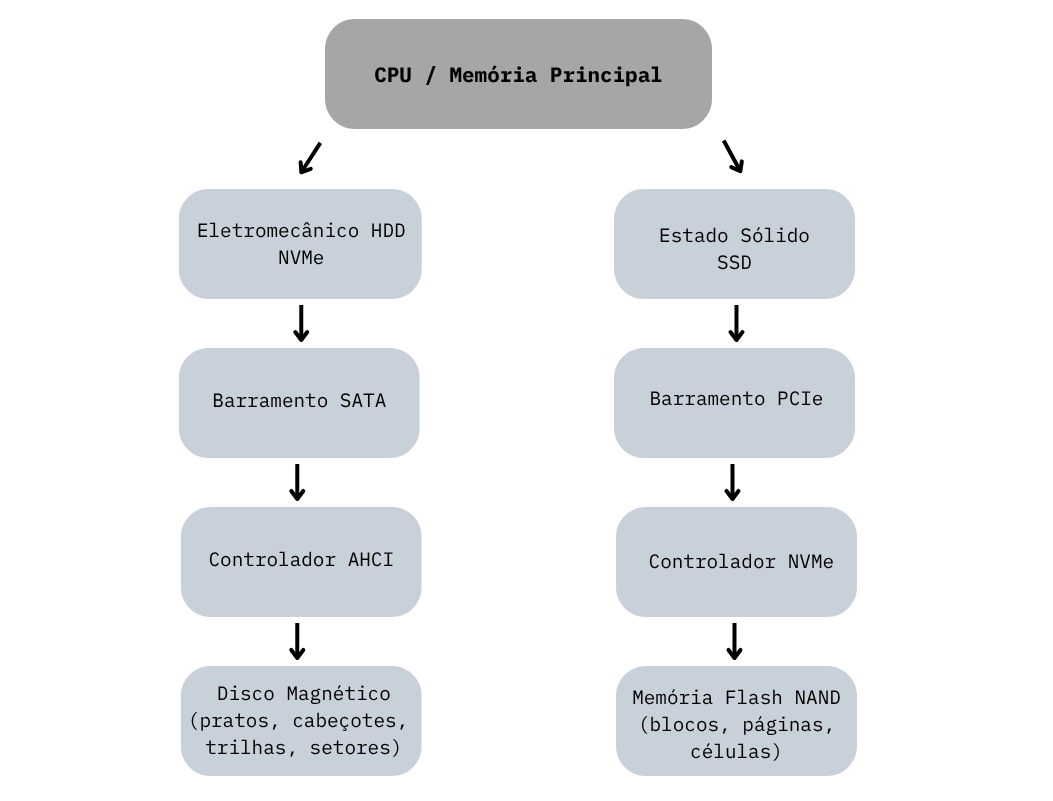
\includegraphics[width=0.7\linewidth]{Diagrama da hierarquia de hardware .png}
    \caption{Diagrama da hierarquia de hardware e do fluxo de dados entre a CPU, a memória RAM e os dispositivos de armazenamento HDD (SATA/AHCI) e SSD (PCIe/NVMe).}
    \label{fig:hierarquia-hardware}
    
    \vspace{2pt}
    \small Fonte: Elaborado pelos autores com base em Stallings (2017).
\end{figure}


O diagrama apresentado na Figura~\ref{fig:hierarquia-hardware} resume a hierarquia de hardware e as duas rotas distintas percorridas pelas requisições de Entrada e Saída (E/S) a partir do subsistema central de processamento (CPU e Memória Principal RAM) \cite{stallings2017}. Na rota mecânica tradicional, os dados trafegam pela interface SATA sob o protocolo AHCI, sendo direcionados até a mídia magnética, onde dependem da movimentação física dos cabeçotes de leitura e gravação sobre os pratos giratórios para localizar as trilhas e setores específicos \cite{oliveira2010, silva2025}. Por outro lado, no caminho de estado sólido moderno, a comunicação ocorre de forma direta através do barramento PCI Express (PCIe) sob o protocolo NVMe, alcançando os chips de memória Flash NAND organizados em blocos, páginas e células semicondutoras \cite{george2023, ribeiro2017}. Dessa forma, o diagrama evidencia a transição arquitetural de um fluxo serializado e dependente de componentes mecânicos para um modelo de alto paralelismo e acesso eletrônico direto \cite{george2023, stallings2017}.

\subsection{Funcionamento Técnico dos Componentes e Mecanismos Lógicos} 
\subsubsection{Discos Magnéticos (HDDs)} 

O funcionamento dos discos rígidos se baseia em um princípio onde pratos circulares cobertos por material ferromagnético giram em alta velocidade em torno de um eixo sob cabeçotes flutuantes \cite{oliveira2010, stallings2017}. O processo de gravação altera a polaridade magnética de domínios microscópicos na superfície do prato por meio de correntes elétricas na bobina do cabeçote, enquanto a leitura é realizada detectando as variações do campo magnético por indução ou por sensores \cite{oliveira2010, stallings2017}. O desempenho de Entrada/Saída (E/S) em um HDD é limitado por dois fatores físicos: o tempo de busca (\textit{seek time}), em relação ao deslocamento mecânico do braço atuador para posicionar o cabeçote sobre a trilha desejada, e a latência rotacional, que representa o tempo de espera para que o setor solicitado gire e se alinhe abaixo do cabeçote \cite{oliveira2010, stallings2017}. 

\subsubsection{Arquitetura SSD (NAND Flash e NVMe)} 

Diferentemente dos HDDs, as Unidades de Estado Sólido (SSDs) utilizam circuitos semicondutores e armazenam dados eletronicamente em arranjos de células de memória Flash NAND \cite{santos2014, stallings2017}. Por não possuírem partes móveis, os SSDs eliminam completamente a busca mecânica e a latência rotacional \cite{santos2014}. Para explorar a velocidade dessas mídias e superar os gargalos de fila única dos antigos protocolos SATA (limitados a 32 comandos), o protocolo NVMe foi projetado especificamente para memórias não voláteis conectadas diretamente ao barramento PCI Express (PCIe) \cite{george2023, xu2015}. A grande inovação do NVMe consiste na introdução de uma arquitetura paralela capaz de suportar até 64.000 filas de comandos (\textit{command queues}), com até 64.000 comandos por fila, permitindo o processamento simultâneo e concorrente de requisições por múltiplos núcleos de CPU \cite{george2023, xu2015}. 

\subsubsection{Mecanismos Lógicos de Gerenciamento (TRIM, Garbage Collection, Wear Leveling e TBW)} 

O gerenciamento do armazenamento em estado sólido baseia-se na cooperação entre o sistema operacional e a controladora interna do dispositivo para administrar a impossibilidade de sobrescrita direta em nível de página \cite{ribeiro2017, santos2014}. Nessa arquitetura, o sistema operacional atua emitindo o comando TRIM para sinalizar à camada de interface quais blocos contêm dados invalidados pelo sistema de arquivos \cite{ribeiro2017, stallings2017}. A partir dessa sinalização, a controladora assume a execução autônoma do processo de Coleta de Lixo (\textit{Garbage Collection}) para reorganizar páginas válidas e liberar blocos limpos, aplicando também rotinas de Nivelamento de Desgaste (\textit{Wear Leveling}) para distribuir as gravações homogeneamente entre as células, o que estabelece a durabilidade nominal do dispositivo expressa pela métrica TBW (\textit{Terabytes Written}) \cite{santos2014, stallings2017}.

\subsection{Análise Comparativa das Tecnologias}
Para sistematizar as diferenças entre as três gerações de dispositivos de armazenamento secundário abordadas nesta pesquisa, foi elaborada uma tabela comparativa baseada em dados operacionais, físicos e arquitetônicos. 


\begin{table}[H]
\vspace{-6pt}
\centering
\caption{Comparativo entre HDDs tradicionais, SSDs SATA e SSDs NVMe.}
\label{tab:comparativo-armazenamento}
\small
\renewcommand{\arraystretch}{1.25}

\begin{tabularx}{\linewidth}{
|>{\raggedright\arraybackslash}p{2.5cm}
|>{\raggedright\arraybackslash}X
|>{\raggedright\arraybackslash}X
|>{\raggedright\arraybackslash}X|}
\hline
\textbf{Categoria} &
\textbf{HDD Tradicional} &
\textbf{SSD SATA (AHCI)} &
\textbf{SSD NVMe (PCIe)} \\
\hline

\textbf{Tecnologia Base} &
Eletromecânica (pratos e cabeçotes magnéticos) &
Eletrônica (semicondutores NAND Flash) &
Eletrônica (semicondutores NAND Flash) \\
\hline

\textbf{Barramento} &
SATA (AHCI) &
SATA (AHCI) &
PCIe (PCI Express) \\
\hline

\textbf{Filas de Comandos} &
1 fila (até 32 comandos) &
1 fila (até 32 comandos) &
Até 64.000 filas de comandos \\
\hline

\textbf{Gerenciamento Lógico} &
Não requer TRIM &
TRIM, Garbage Collection e Wear Leveling &
TRIM, Garbage Collection e Wear Leveling \\
\hline

\textbf{Métrica de Durabilidade} &
MTBF (horas de uso) &
TBW (Terabytes Written) &
TBW (Terabytes Written) \\
\hline

\textbf{Taxa de Transferência} &
Aproximadamente 80 a 200 MB/s &
Aproximadamente 500 a 550 MB/s &
Aproximadamente 3.000 a 7.500+ MB/s \\
\hline

\textbf{Latência Média} &
Alta &
Baixa &
Extremamente baixa \\
\hline
\end{tabularx}

\vspace{2mm}
\begin{flushleft}
\footnotesize
Fonte: Elaborado pelos autores com base em Silva et al. (s.d.),
George et al. (s.d.) e Stallings (2017).
\end{flushleft}
\end{table}

Ao analisar os dados da Tabela 1, nota-se o salto na taxa de transferência de dados e a redução da latência ao migrar da tecnologia eletromecânica para os SSDs NVMe. Enquanto o HDD tradicional fica limitado pelo deslocamento mecânico e o SSD SATA permanece estagnado pelo gargalo de fila única do protocolo AHCI, a arquitetura NVMe alcança throughputs até 35 vezes maiores aos dos discos magnéticos e latências na ordem de microssegundos. Esse avanço é impulsionado pelo paralelismo de filas de comandos no barramento PCIe, demonstrando que a superação dos gargalos do armazenamento moderno depende tanto da velocidade dos chips Flash NAND quanto de protocolos de interconexão otimizados.

\section{Análise Crítica e Gargalos Arquiteturais}

\subsection{Limitações físicas e arquiteturais dos dispositivos HDD e SSD}

Os HDDs e os SSDs apresentam diferenças estruturais que afetam a forma como os dados são armazenados e acessados. Nos discos rígidos, as informações são registradas magneticamente em discos que permanecem em movimento durante o funcionamento do dispositivo, enquanto cabeças de leitura e gravação realizam o acesso aos dados. A necessidade desses movimentos físicos pode aumentar o tempo de resposta, sobretudo quando as informações estão distribuídas em diferentes regiões do disco. Em contrapartida, os SSDs armazenam os dados em células de memória Flash não volátil e realizam o acesso eletronicamente, sem depender de peças móveis. Essa arquitetura contribui para diminuir a latência e oferece maior resistência a impactos e vibrações.

\begin{figure}[H]
  \centering
  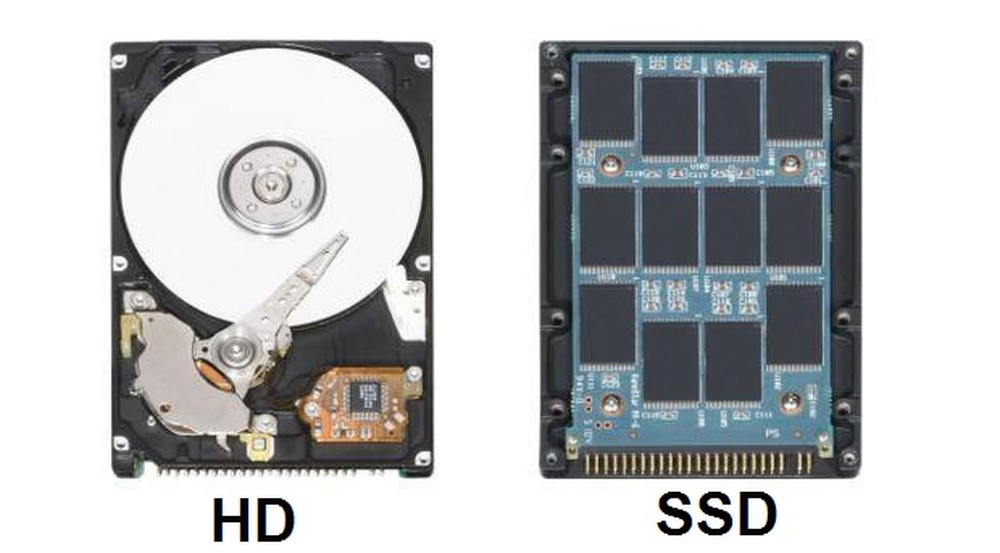
\includegraphics[width=0.5\linewidth]{2013-10-22-ssdvhd.jpg}
  \caption{Comparação entre as estruturas físicas de um HDD e um SSD}
  {\small \textbf{Fonte:} \cite{coutinho2013}}
  \label{fig:comparacao_hdd_ssd}
\end{figure}

O desempenho também é influenciado pela forma como o dispositivo se comunica com os demais componentes do computador. Enquanto os HDDs e os SSDs SATA utilizam a interface SATA, os SSDs NVMe geralmente se conectam por meio do barramento PCI Express (PCIe). Desenvolvido especificamente para dispositivos de armazenamento não volátil, o NVMe oferece suporte a múltiplas filas de comandos, favorecendo o processamento simultâneo de solicitações. Ainda assim, o desempenho obtido depende das características do dispositivo e da infraestrutura em que ele opera \cite{nvmexpress2026}.

\subsection{Latência e gargalos de desempenho}

A latência é um dos fatores que ajudam a explicar as diferenças de desempenho
entre os dispositivos de armazenamento secundário. Nos discos rígidos (HDDs), o teto físico imposto pelos componentes mecânicos resulta em um gargalo severo de Entrada e Saída por Segundo (IOPS), sobretudo sob padrões de acesso aleatório (\textit{random access}), nos quais as solicitações concorrentes forçam constantes reposicionamentos dos cabeçotes e elevam o tempo total de resposta do sistema \cite{stallings2017}. 
Em contrapartida, a arquitetura de estado sólido elimina a latência mecânica ao realizar acessos eletrônicos diretos às células de memória Flash, reduzindo os tempos de resposta para a escala de microssegundos \cite{stallings2017}. No entanto, o desempenho global do SSD não é determinado apenas pela latência nominal da mídia, dependendo fortemente da taxa de transferência do controlador, do tipo de célula NAND e da eficiência do protocolo de comunicação \cite{stallings2017}. 
Nesse contexto, a adoção do protocolo NVMe sobre o barramento PCIe resolve o gargalo de \textit{software} historicamente imposto pelas interfaces herdadas, ao introduzir o processamento paralelo em múltiplas filas de comandos. Essa arquitetura minimiza a sobrecarga de interrupções no processador e otimiza a vazão em sistemas \textit{multithreaded}; contudo, os ganhos reais de velocidade permanecem condicionados ao padrão de acesso da aplicação e à infraestrutura em que o dispositivo opera \cite{nvmexpress2026}.

\subsection{Trade-offs entre desempenho, custo e capacidade}
A seleção de tecnologias no subsistema de armazenamento secundário envolve compromissos necessários (\textit{trade-offs}) entre desempenho, capacidade e custo por unidade de armazenamento. Os SSDs NVMe oferecem tempos de acesso na ordem de microssegundos e altas taxas de IOPS, otimizando o carregamento de sistemas operacionais, bancos de dados transacionais e aplicações de tempo real \cite{stallings2017}. Em contrapartida, os HDDs mantêm relevância econômica pelo menor custo por gigabyte, sendo vantajosos para o armazenamento massivo em infraestruturas de grande porte \cite{silva2025}. Para equilibrar essa relação custo-benefício, adota-se a arquitetura de armazenamento em camadas. Nesse modelo, os SSDs são posicionados em níveis superiores de \textit{cache} para alocação de dados frequentemente acessados (\textit{hot data}), enquanto os HDDs atuam no armazenamento em massa de menor custo, combinando a baixa latência da memória Flash com a alta densidade magnética \cite{santos2014, oliveira2010}.

\subsection{TRIM, desgaste da memória flash e TBW}
Embora o gerenciamento lógico mitigue a degradação operacional, a arquitetura da memória Flash NAND enfrenta gargalos físicos intrínsecos resultantes do estresse elétrico no dielétrico da célula semicondutora \cite{santos2014, stallings2017}. A aplicação repetida de pulsos de alta tensão necessários para os ciclos de apagamento provoca a degradação progressiva da camada de óxido, comprometendo a capacidade de retenção de carga elétrica e impondo um limite finito de ciclos de Programação/Apagamento (P/E) \cite{santos2014, stallings2017}. Além disso, a execução de rotinas em segundo plano, como a Coleta de Lixo (\textit{Garbage Collection}) e o Nivelamento de Desgaste (\textit{Wear Leveling}), acarreta o fenômeno da Amplificação de Escrita (\textit{Write Amplification}), no qual o volume de gravações físicas executadas na mídia supera o volume solicitado pelas aplicações, elevando a latência e penalizando o desempenho sob cargas intensivas \cite{santos2014}. 

Nesse cenário de degradação temporal, o comando TRIM atua como um mecanismo crítico de otimização, permitindo que o sistema operacional informe de maneira antecipada os blocos invalidados pelo sistema de arquivos, o que reduz o fator de amplificação de escrita e atenua quedas severas na taxa de transferência do dispositivo \cite{ribeiro2017, stallings2017}. A partir da combinação desses fatores de estresse físico e mitigações lógicas, os fabricantes estabelecem o teto de durabilidade comercial da mídia parametrizado pela métrica TBW (\textit{Terabytes Written}), que quantifica o volume acumulado de gravações suportado antes que o desgaste do dielétrico comprometa a integridade dos dados \cite{stallings2017}.


\section{Considerações Finais}

O presente artigo \textit{survey} analisou a evolução do subsistema de armazenamento secundário na arquitetura de computadores, evidenciando como a transição dos dispositivos eletromecânicos para mídias de estado sólido redefiniu os parâmetros de desempenho e os gargalos do sistema \cite{stallings2017, silva2025}. 

Enquanto os discos rígidos (HDDs) permanecem limitados pelas restrições físicas do movimento de braços atuadores e da latência rotacional, a adoção das Unidades de Estado Sólido (SSDs) superou o gargalo de fila única dos controladores AHCI/SATA e viabilizou o paralelismo com múltiplas filas de comandos \cite{george2023}. Por outro lado, a análise crítica demonstrou que a tecnologia Flash NAND introduz desafios lógicos e físicos próprios, tais como a impossibilidade de sobrescrita direta (\textit{erase before write}), o estresse elétrico do dielétrico por pulsos de alta tensão, o fenômeno da amplificação de escrita (\textit{write amplification}) e a limitação da vida útil mensurada em TBW (\textit{Terabytes Written}) \cite{ribeiro2017, santos2014}. 

Diante desses fatores, conclui-se que a substituição integral da tecnologia magnética permanece inviável em cenários de armazenamento massivo, consolidando a hierarquização e os sistemas híbridos como a abordagem de melhor relação custo-benefício para a infraestrutura de computadores \cite{santos2014, silva2025}. 

Para o futuro do armazenamento secundário, apontam-se como tendências a expansão das larguras de banda proporcionadas pelas novas gerações do barramento PCIe, a consolidação do \textit{NVMe over Fabrics} (NVMe-oF) para desagregação e compartilhamento de arranjos \textit{flash} em rede e a adoção do armazenamento computacional (\textit{computational storage}) para processamento local de dados \cite{george2023}. Adicionalmente, o amadurecimento de novas memórias não voláteis de alta densidade como ReRAM, PCRAM e STT-RAM aponta para a redução da lacuna de latência entre a memória principal (DRAM) e a memória externa, garantindo que a inovação em protocolos e no gerenciamento lógico continuará a impulsionar o desempenho e a eficiência energética dos sistemas digitais \cite{stallings2017}.

\section{Referências}


\bibliographystyle{sbc}
\bibliography{referencias}

\end{document}
